\chapter{Генерация изображений с помощью методов машинного обучения}
\section{U-Net}
\section{Диффузионные нейронные сети для генерации изображений}
\section{Латентные диффузионные нейронные сети для генерации изображений}

Генерация изображений с помощью нейронных сетей сегодня играет важную роль в развитии
информационных технологий, позволяя автоматизировать создание иллюстраций.
Широкое распространение генеративных технологий стало возможно благодаря улучшению методов обучения нейронных
сетей, которые решают данную задачу, и развитию вычислительной техники.

Одним из значимых методов обучения нейронных сетей, предназначенных для генерации изображений, стал Generative adversarial network (GAN).
Ключевой особенностью данного метода на этапе обучения является наличие двух глубоких нейронных сетей: $G(z)$, которая по распределению $p_g$ ставит
в соответствие векторам $z$ изображения $x$, и сети $D(x)$, которая возвращает скалярное значение,
которое является вероятностью того, что $x$ является реальным изображением, то есть является частью
обучающей выборки. 
Основная идея процесса обучения заключается в минимизации величины $\log (1 - D(G(z)))$, что означает, что $G$ пытается «обмануть» дискриминатор $D$,
что не требует привлечения учителя. 

Таким образом процесс получения распределения $p_g$ можно представить в виде игры с нулевой суммой двух игроков
с критерием 
$$
\min_{G}\max_{D} V(D, G) = \mathbf{E}_{x~p_{data}(x)}[\log D(x)] + \mathbf{E}_{z~p_{z}(z)}[\log (1 - D(G(z)))]
$$ 

Данный подход гарантирует сходимость при увеличении обучающей выборки и обеспечивает хорошую скорость инференса относительно подходов,
основанных на других вероятностных методах, но является очень трудозатратным при обучении модели.


\begin{figure}[H]
  \centering
  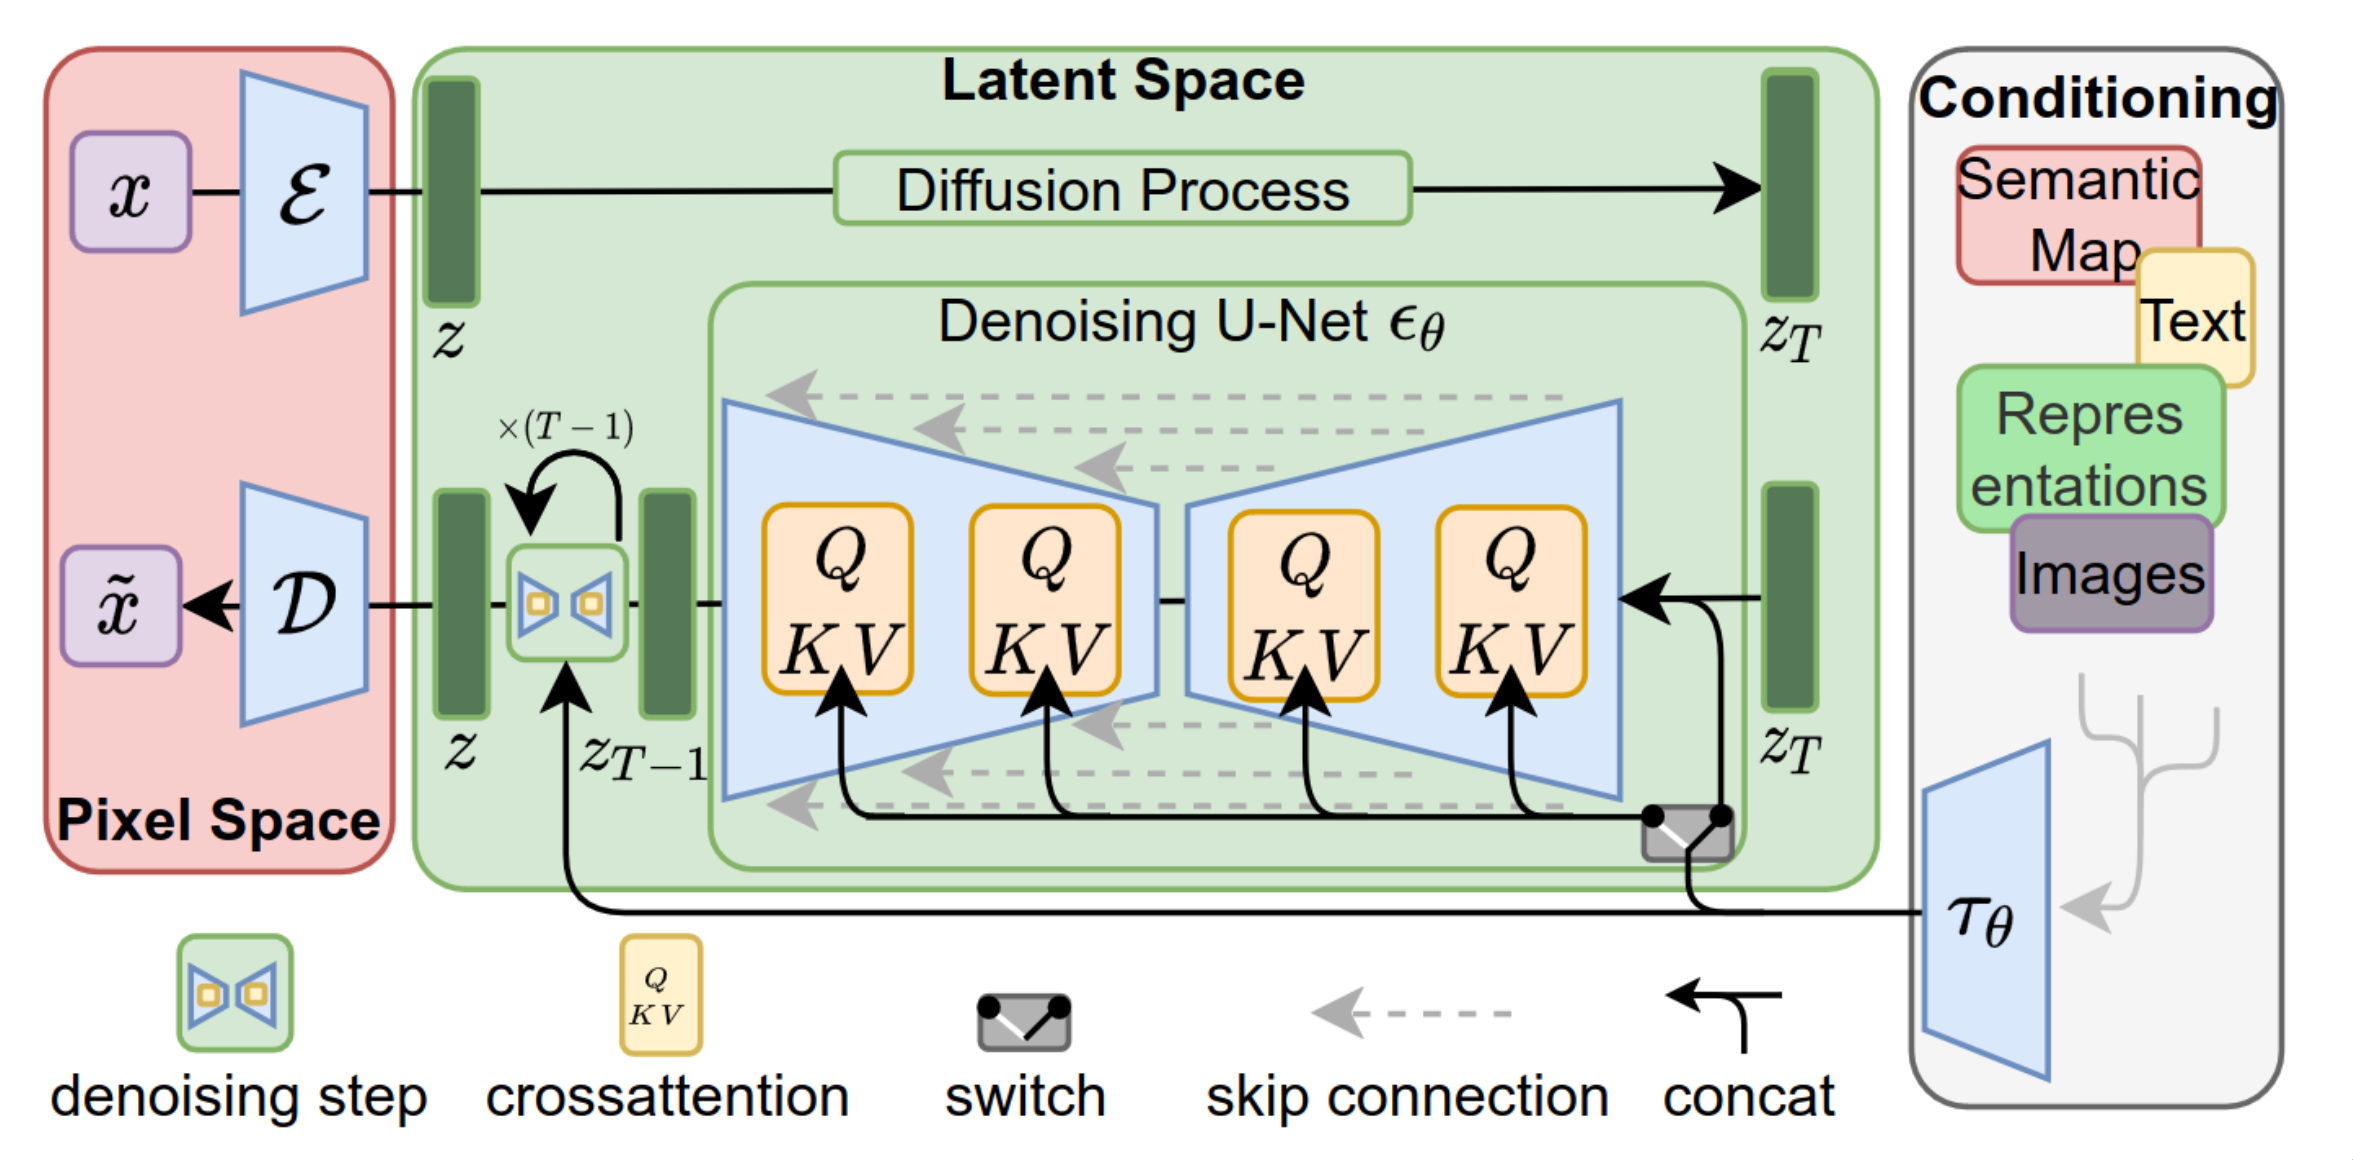
\includegraphics[width=0.95\textwidth]{img/latent.png}
  \caption{Схема архитектуры \cite{rombach2022high}}
    \label{fig:latent}
\end{figure}